%%%%%%%%%%%%%%%%%%%%%%%%%%%%%%%%%%%%%%%%%
% Undergraduate Project Report Template
% University of Mines and Technology (UMaT), Tarkwa
% Based on template by Dr Hamidu Abdel-Fatao and Dr Stephen Anokye
%%%%%%%%%%%%%%%%%%%%%%%%%%%%%%%%%%%%%%%%%

%----------------------------------------------------------------------------------------
%	PACKAGES AND DOCUMENT CONFIGURATION
%----------------------------------------------------------------------------------------

\documentclass[12pt, onehalfspacing, liststotoc, oneside, parskip, headsepline,UKenglish]{UMaT_Undergrauate_Report_Template_Configurations}

\setlength{\parskip}{1em}
\setlength{\parindent}{0pt}
\usepackage[a4paper, top=1in, bottom=1in, left=1.2in, right=1in]{geometry}

\usepackage[utf8]{inputenc}
\usepackage[T1]{fontenc}
\usepackage{newtxtext,newtxmath}
\usepackage{subcaption}
\usepackage{etoolbox}
\patchcmd{\endabstract}{\null}{}{}{}
\usepackage{pgfplots}
\pgfplotsset{compat=1.18}
\usepgfplotslibrary{statistics}
\usepackage{times}

% Language-aware quoting (required by biblatex)
\usepackage[autostyle=true]{csquotes}

% Bibliography
\usepackage[
    backend=biber,
    style=authoryear,
    natbib=true,
    uniquename=false,
    uniquelist=false,
    maxcitenames=3,
    maxbibnames=999,
    giveninits=true,
    dashed=false,
    sorting=nyt,
    url=false,
    doi=false,
    isbn=false,
    eprint=false
]{biblatex}

\DeclareNameAlias{sortname}{family-given}
\DeclareDelimFormat{nameyeardelim}{\addcomma\space}
\renewbibmacro*{date+extrayear}{%
    \setunit{\addcomma\space}%
    \printtext[parens]{%
        \printfield{labelyear}%
        \printfield{extrayear}}}
\DeclareFieldFormat{sentencecase}{#1}
\renewcommand{\newunitpunct}{\addcomma\space}
\renewbibmacro{in:}{}
\DeclareFieldFormat[
    article,
    inbook,
    incollection,
    inproceedings,
    misc,
    online,
    report,
    thesis,
    unpublished
]{title}{\textquotedblleft#1\textquotedblright}
\addbibresource{references.bib}

% Italicise "et al." in citations
\usepackage{xpatch}
\xpatchbibmacro{name:andothers}{%
    \bibstring{andothers}%
}{%
    \bibstring[\emph]{andothers}%
}{}{}

% Chapter/section formatting
\usepackage{titlesec, titletoc}
\titleformat{\chapter}[display]
  {\fontsize{14}{24} \bfseries \centering}{\MakeUppercase{\chaptertitlename}\ \thechapter}{0pt}{\normalsize \MakeUppercase}
\titlespacing*{\chapter}{-10pt}{-45pt}{25pt}

% Custom commands
\newcommand{\keyword}[1]{\textbf{#1}}
\newcommand{\tabhead}[1]{\textbf{#1}}
\newcommand{\code}[1]{\texttt{#1}}
\newcommand{\file}[1]{\texttt{\bfseries#1}}
\newcommand{\modelname}{\texttt{rmanluo/\allowbreak GCR-\allowbreak Meta-\allowbreak Llama-\allowbreak 3.1-\allowbreak 8B-\allowbreak Instruct}}
\newcommand{\option}[1]{\texttt{\itshape#1}}
\renewcommand{\indexname}{INDEX}

% Bordered table helpers
\newenvironment{gridtabular}[1]{\begin{tabular}{|#1|}\hline}{\end{tabular}}
\newcommand{\gr}[1]{#1\\\hline}

% Graphics
\usepackage{graphicx}
\graphicspath{{./res/}}

% Tables, lists, floats
\usepackage{enumitem}
\usepackage{array}
\usepackage{tabularx}
\usepackage{float}
\usepackage{longtable}
\usepackage{microtype}
\usepackage{etoc}
\usepackage{ltablex}
\keepXColumns
\usepackage{multirow}
\usepackage{tocloft}
\usepackage{hyphenat}
\usepackage{lipsum}
\usepackage[nottoc,numbib]{tocbibind}
\usepackage{hyperref}
\usepackage{xcolor}
\usepackage{caption}

% TikZ, algorithms, landscape
\usepackage{pgfgantt}
\usepackage{tikz}
\usepackage{algorithm}
\usepackage{algpseudocode}
\usetikzlibrary{arrows.meta}
\usepackage{pdflscape}
\usepackage{setspace}

% Hyperlink colours
\hypersetup{
  colorlinks=true,
  linkcolor=black,
  urlcolor=black,
  citecolor=black,
  pdfborder={0 0 0}
}

% Additional bibliography formatting
\DeclareFieldFormat[article]{volume}{\addcomma\space Vol.~#1,\addspace}
\DeclareFieldFormat[article]{number}{\space No.~#1}

\setlength{\cftfignumwidth}{7em}
\setlist[enumerate]{itemsep=0.2em, parsep=0pt}

% List of Figures customisation
\renewcommand{\cftfigfont}{\normalfont\centering}
\renewcommand{\cftfigpagefont}{\hfill}
\renewcommand{\cftfigleader}{\cftdotfill{\cftsecdotsep}}
\renewcommand{\cftdotsep}{\cftnodots}
\setlength{\cftfigindent}{0pt}
\setlength{\cftbeforefigskip}{4pt}
\renewcommand{\cftfigaftersnumb}{\quad}
\setlength{\cftfignumwidth}{10em}

% Chapter numbering in ToC
\makeatletter
\renewcommand{\@chapter}[2][]{%
  \ifnum \c@secnumdepth >\m@ne
    \if@mainmatter
      \refstepcounter{chapter}%
      \typeout{\@chapapp\space\thechapter.}%
      \addcontentsline{toc}{chapter}%
        {\protect\numberline{\thechapter}#1}%
    \else
      \addcontentsline{toc}{chapter}{#1}%
    \fi
  \else
    \addcontentsline{toc}{chapter}{#1}%
  \fi
  \chaptermark{#1}%
  \addtocontents{lof}{\protect\addvspace{0\p@}}%
  \addtocontents{lot}{\protect\addvspace{0\p@}}%
  \if@twocolumn
    \@topnewpage[\@makechapterhead{#2}]%
  \else
    \@makechapterhead{#2}%
    \@afterheading
  \fi}
\makeatother

% Caption formatting
\captionsetup[figure]{labelfont={bf},textfont={bf}}
\captionsetup[table]{
    justification=raggedright,
    singlelinecheck=off,
    format=plain,
    labelsep=space,
    width=\textwidth,
    margin={0pt,0pt}
}

% Reset figure font overrides
\renewcommand{\cftfigfont}{}
\renewcommand{\cftfigpagefont}{}

% List of Tables customisation
\renewcommand{\cfttabindent}{0pt}
\setlength{\cftbeforetabskip}{4pt}
\setlength{\cfttabnumwidth}{12em}

% CHAPTER label in ToC
\renewcommand{\cftchappresnum}{CHAPTER\space}
\renewcommand{\cftchapnumwidth}{7em}

\makeatletter
\setlength{\@fptop}{0pt}
\makeatother

% Section formatting
\titleformat{\section}
{\normalfont\normalsize\bfseries}{\thesection}{1em}{}
\titleformat{\subsection}
{\normalfont\normalsize}{\thesubsection}{1em}{}
\titleformat{\subsubsection}
{\normalfont\normalsize\itshape}{\thesubsubsection}{1em}{}

%----------------------------------------------------------------------------------------
%	THESIS INFORMATION
%----------------------------------------------------------------------------------------

\thesistitle{A Thesis Report Entitled}
\examiner{}
\degree{}
\author{Your Full Name}
\addresses{}
\keywords{}
\university{\href{https://www.umat.edu.gh/}{\large  UNIVERSITY OF MINES AND TECHNOLOGY, TARKWA}}
\department{{\large DEPARTMENT OF COMPUTER SCIENCE AND ENGINEERING }}
\group{}
\faculty{{\large FACULTY OF COMPUTING AND MATHEMATICAL SCIENCES}}

\AtBeginDocument{
\hypersetup{pdftitle=\ttitle}
\hypersetup{pdfauthor=\authorname}
}

\linespread{1.5}

\DeclareCaptionLabelSeparator{mysep}{\hspace{0.2cm}  }
\captionsetup{format=plain, font=normalfont, labelfont=bf, labelsep=mysep}


\begin{document}

\frontmatter

\pagestyle{plain}

%----------------------------------------------------------------------------------------
%	TITLE PAGE
%----------------------------------------------------------------------------------------

\begin{titlepage}
  \large
  \begin{center}

    {\scshape \univname\par}\vspace{0cm}

    { FACULTY OF  COMPUTING AND MATHEMATICAL SCIENCES}\\[0.02cm]

    {  DEPARTMENT OF COMPUTER SCIENCE AND ENGINEERING }\\[0.8cm]

    \vspace{0.2cm}
    {  A PROJECT REPORT ENTITLED }\\[0.1cm]
    {  DYNAMIC CONTEXT-AWARE TRIES FOR KNOWLEDGE GRAPH-CONSTRAINED LARGE LANGUAGE MODEL GENERATION}\\[1cm]

    {  BY}\\
    { BERNARD KIRK ADJANOR KATAMANSO}\\
    { ERICA AMONOR}\\
    { JOSEPH OSEI NYARKO}\\
    { JESSICA AFUA ETORNAM NSAFOAH}\\[1.2cm]

    {  SUBMITTED IN PARTIAL FULFILMENT OF THE REQUIREMENT FOR THE AWARD OF THE DEGREE OF BACHELOR OF SCIENCE IN COMPUTER SCIENCE AND ENGINEERING }\\[1.2cm]

    {  PROJECT SUPERVISOR}\\[0.3cm]

    .............................................................\\

    {  DR ERIC AFFUM}\\[0.6cm]
    {  TARKWA, GHANA\\ August 2026}

  \end{center}
\end{titlepage}

%----------------------------------------------------------------------------------------
%	DECLARATION PAGE
%----------------------------------------------------------------------------------------
\vspace{-20pt}
\begin{declaration}
  \addchaptertocentry{\authorshipname}

  We, BERNARD KIRK ADJANOR KATAMANSO, ERICA AMONOR, JOSEPH OSEI NYARKO and JESSICA AFUA ETORNAM NSAFOAH, declare that this project work is our own original work. It is being submitted for the degree of Bachelor of Science in Computer Science and Engineering at the University of Mines and Technology (UMaT), Tarkwa. It has not been submitted, either in whole or in part, for any degree or examination at any other university.\vspace{20pt}

  Name: \qquad KATAMANSO BERNARD KIRK ADJANOR \vspace{-0.2pt}

  \noindent Signature: \rule{7cm}{0.8pt}\\

  Name: \qquad AMONOR ERICA\vspace{-0.2pt}

  \noindent Signature: \rule{7cm}{0.8pt}\\

  Name: \qquad  NYARKO JOSEPH OSEI \vspace{-0.2pt}

  \noindent Signature: \rule{7cm}{0.8pt}\\

  Name: \qquad NSAFOAH JESSICA AFUA ETORNAM \vspace{-0.2pt}

  \noindent Signature: \rule{7cm}{0.8pt}\\

  \vspace{0.8cm}

  \hspace{5.3em} day of\vspace{-10pt} \hspace{9em} (year)\vspace{-5pt}

  \noindent \rule[0.5em]{5em}{0.5pt} \hspace{3.5em} \rule[0.5em]{8em}{0.5pt} \hspace{3.2em} \rule[0.5em]{5em}{0.5pt}
\end{declaration}

%----------------------------------------------------------------------------------------
%	ABSTRACT PAGE
%----------------------------------------------------------------------------------------

\begin{abstract}
  \vspace{10pt}
  \addchaptertocentry{\abstractname}
  Knowledge Graph constrained decoding eliminates hallucination in large language model (LLM) reasoning by restricting output to verified paths. The leading approach, Graph Constrained Reasoning (GCR), achieves zero hallucination on Knowledge Graph Question Answering (KGQA) benchmarks by encoding all structurally valid paths in a static trie. The constraint is absolute but indifferent to the question: a three-hop query with twenty out-degree relations admits roughly 24{,}000 paths, and the LLM must navigate among them using the same internal knowledge that causes hallucination. We introduce Dynamic Context-Aware Tries (DCA-Trie), a dynamic constrained decoding framework that prunes the valid path set during generation using a TypeOracle, a lightweight symbolic module that checks two ontology gates per candidate triple. On a controlled 300-question WebQSP subset, DCA-Trie removes 13.8\% of semantically irrelevant paths while maintaining a false negative rate below 5\%. We further introduce the Semantic Irrelevance Ratio (SIR), a metric that separates constraint quality from answer accuracy, enabling independent evaluation of what the oracle filters versus what the LLM actually uses. SIR reveals a non-monotone relationship between constraint tightness and answer correctness: tighter constraints reduce the search space but do not improve Hits@1 (4.0pp lower for the static variant, 4.7pp for the lazy variant), while a per-hop architectural variant collapses by 25 points regardless of its gates. We show that the accuracy cost is attributable to the gates themselves via calibration, and that the lazy variant recovers the efficiency of dynamic adaptation in a single, stable decoding pass. DCA-Trie and SIR together provide the first framework for independently evaluating constraint quality and answer accuracy in knowledge graph-constrained decoding.

\end{abstract}

%----------------------------------------------------------------------------------------
%	DEDICATION
%----------------------------------------------------------------------------------------

\begin{dedication}
  \vspace{10pt}
  \centering
  Dedicated to our parents. For every sacrifice we didn't see and every kindness we never had to ask for. Thank you for everything.
\end{dedication}

%----------------------------------------------------------------------------------------
%	ACKNOWLEDGEMENTS
%----------------------------------------------------------------------------------------

\begin{acknowledgements}
  \addchaptertocentry{\acknowledgementname}
  \vspace{0.5cm}
  We thank Dr. Eric Affum for his guidance, patience, and support throughout this project. His supervision was instrumental in shaping the direction of this work. We also express our appreciation to our families, friends, and mentors for their encouragement and understanding throughout the process. Finally, we acknowledge the academic community whose work has informed and inspired this research. This dissertation builds on the contributions of many scholars, and we are grateful for their work.
\end{acknowledgements}
\pagebreak

%----------------------------------------------------------------------------------------
%  TABLE OF CONTENTS / LIST OF FIGURES / LIST OF TABLES
%----------------------------------------------------------------------------------------
\phantomsection
\vspace*{60pt}
\addcontentsline{toc}{chapter}{TABLE OF CONTENTS}
\vspace{10pt}
\renewcommand{\contentsname}{\hfill\large\bfseries TABLE OF CONTENTS\hfill}
\vspace{-5ex}

\textbf{Contents} \hspace{0.84\textwidth} \textbf{Page}

\vspace*{-4cm}

\setlength{\cftsecindent}{0pt}
\setlength{\cftsubsecindent}{2.2em}
\tableofcontents
\pagebreak

\newpage
\makeatletter
\vspace{10pt}
\chapter*{\large\bfseries\centering\vspace{15pt} LIST OF FIGURES}
\addcontentsline{toc}{chapter}{LIST OF FIGURES}
\phantomsection
\vspace{-4ex}
\textbf{Figure} \hspace{0.4\textwidth} \textbf{Title} \hspace{0.4\textwidth} \textbf{Page}
\vspace{-3ex}
\@starttoc{lof}
\makeatother
\clearpage

\makeatletter
\titlecontents{figure}
[0pt]
{}
{\MakeUppercase{Fig.~\thecontentslabel\quad Title Page}\quad}
{}
{\titlerule*[0.5pc]{.}\contentspage}

\vspace{10pt}
\chapter*{\large\bfseries\centering\vspace{15pt} LIST OF TABLES}
\addcontentsline{toc}{chapter}{LIST OF TABLES}
\phantomsection
\vspace{-4ex}
\textbf{Table} \hspace{0.4\textwidth} \textbf{Title} \hspace{0.4\textwidth} \textbf{Page}
\vspace{0.2cm}
\@starttoc{lot}
\makeatother

\clearpage

%----------------------------------------------------------------------------------------
%	LIST OF ABBREVIATIONS
%----------------------------------------------------------------------------------------
\chapter*{\large\centering\vspace{15pt}LIST OF ABBREVIATIONS}
\addcontentsline{toc}{chapter}{LIST OF ABBREVIATIONS}
\vspace{-4ex}
\vspace{2ex}

\textbf{Abbreviation} \hspace{0.235\textwidth} \textbf{Meaning}
\begin{description}[style=nextline,leftmargin=4.5cm,labelwidth=4cm,font=\normalfont,itemsep=-1.5ex]

  \item[AI]\hspace{0.1\textwidth} Artificial Intelligence
  \item[BFS]\hspace{0.1\textwidth} Breadth-First Search
  \item[CoT]\hspace{0.1\textwidth} Chain-of-Thought
  \item[CWQ]\hspace{0.1\textwidth} ComplexWebQuestions
  \item[DCA-Trie]\hspace{0.1\textwidth} Dynamic Context-Aware Trie
  \item[DoG]\hspace{0.1\textwidth} Decoding on Graphs
  \item[FNR]\hspace{0.1\textwidth} False Negative Rate
  \item[FSM]\hspace{0.1\textwidth} Finite State Machine
  \item[GCD]\hspace{0.1\textwidth} Grammar-Constrained Decoding
  \item[GCR]\hspace{0.1\textwidth} Graph-Constrained Reasoning
  \item[GNN]\hspace{0.1\textwidth} Graph Neural Network
  \item[GPU]\hspace{0.1\textwidth} Graphics Processing Unit
  \item[KG]\hspace{0.1\textwidth} Knowledge Graph
  \item[KGQA]\hspace{0.1\textwidth} Knowledge Graph Question Answering
  \item[LLM]\hspace{0.1\textwidth} Large Language Model
  \item[NLP]\hspace{0.1\textwidth} Natural Language Processing
  \item[QA]\hspace{0.1\textwidth} Question Answering
  \item[RAG]\hspace{0.1\textwidth} Retrieval-Augmented Generation
  \item[RLHF]\hspace{0.1\textwidth} Reinforcement Learning from Human Feedback
  \item[SBERT]\hspace{0.1\textwidth} Sentence Bidirectional Encoder
  \item[] \hspace{0.1\textwidth} Representations from Transformers
  \item[SIR]\hspace{0.1\textwidth} Semantic Irrelevance Ratio
  \item[SQL]\hspace{0.1\textwidth} Structured Query Language
  \item[VRAM]\hspace{0.1\textwidth} Video Random Access Memory

\end{description}

%----------------------------------------------------------------------------------------
%	THESIS CONTENT - CHAPTERS
%----------------------------------------------------------------------------------------

\mainmatter

\pagestyle{thesis}

/home/bernard/research/projects/FINAL_PROJECT/chapters/Chapter1_Introduction.tex % Introduction
/home/bernard/research/projects/FINAL_PROJECT/chapters/Chapter2_Literature_Review.tex % Literature Review
/home/bernard/research/projects/FINAL_PROJECT/chapters/Chapter3_Methodology.tex % Methodology
% Chapter 4

\chapter{RESULTS AND DISCUSSION} % Main chapter title

\label{Chapter4} % For referencing the chapter elsewhere, use \ref{Chapter4} 

    The purpose of this chapter is to present the implementation and results of the .......................................

\section{Testing of Overall System}
    \lipsum[5]

    \begin{figure}[H]
        \centering
        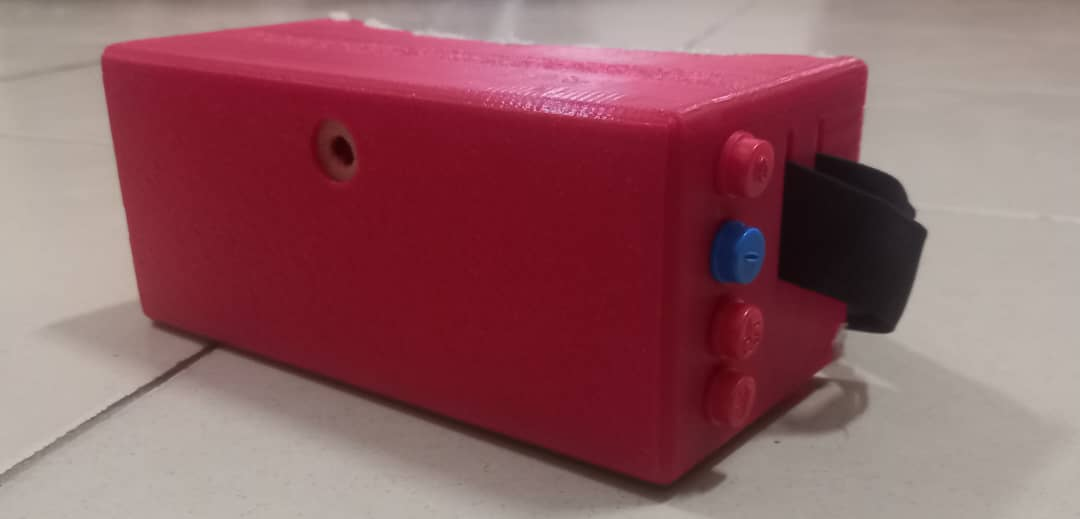
\includegraphics[width=1\textwidth]{Figures/device.jpg}
        \caption{Headwear Device during Startup and Connection}
        \label{fig:system-startup}
    \end{figure}

    

\section{Results}
    \lipsum[5]


 
 % Results and Discussion
% Chapter 5
\chapter{CONCLUSION AND RECOMMENDATIONS} % Main chapter title
\label{Chapter5} % For referencing the chapter elsewhere, use \ref{Chapter5}

\section{Conclusion}
The AI-powered headwear ............................................

\section{Recommendations}
Based on the findings and feedback from testing, ..............................
 % Conclusion and Recommendations

%----------------------------------------------------------------------------------------
%	THESIS CONTENT - APPENDICES
%----------------------------------------------------------------------------------------

\appendix
\addcontentsline{toc}{chapter}{Appendices}

% =============================================================================
% APPENDIX C: ABANDONED SCORER DESIGNS
% =============================================================================

\chapter{Abandoned Semantic Scorer Designs}
\label{AppendixC}

This appendix gives the full design rationale for the two embedding-based relevance scorers (Approaches 1 and 2) that preceded the final symbolic TypeOracle described in Chapter~3, Section~\ref{sec:ch3scorer}. Both designs were implemented and tested before being abandoned in favour of the ontology-gate formulation.

\section{Approach 1: Cosine Similarity (Abandoned)}

The initial design scored each candidate path by computing cosine similarity between a sentence-transformer embedding of the serialised path string and an embedding of the input question:
\begin{equation}
  \text{score}(p, q) = \cos\!\bigl(E(\text{str}(p)),\; E(q)\bigr)
  \label{eq:appc_cosine_v1}
\end{equation}
A path was admitted if $\text{score}(p, q) \geq \tau$, where $\tau$ was a tuned threshold. This approach was abandoned for four reasons:

\begin{enumerate}
  \item \textit{Semantic collapse:} A single cosine score cannot distinguish \textit{why} a path is relevant. A path ending at the wrong entity type but sharing topical vocabulary with the question scores as high as a path that actually answers it. Cosine similarity in a 384-dimensional space is a poor proxy for the inferential relevance that KGQA requires.
  \item \textit{Encoder cost:} Every candidate path requires a full forward pass through \texttt{all-MiniLM-L6-v2}. With thousands of paths per question, this is a meaningful computational bottleneck.
  \item \textit{Threshold sensitivity:} The admission threshold $\tau$ is dataset-dependent and must be tuned on a validation split. Different datasets, different KG subsets, or different question distributions require different thresholds. At $\tau = 0.25$, 84\% of WebQSP queries produced empty path sets after filtering: the threshold was so aggressive that it rejected nearly all paths, leaving the LLM with nothing to generate. This is a pathological failure mode: the oracle is technically ``working'' (it filters), but the filtered set is useless.
  \item \textit{Non-determinism:} Floating-point cosine similarity introduces non-deterministic admission decisions across runs, making the oracle difficult to reproduce exactly.
\end{enumerate}

\section{Approach 2: Decomposed Product Score (Abandoned)}

The second design replaced the monolithic cosine score with a product of three interpretable components:
\begin{equation}
  \text{score}(e_t, r, e' \mid q) = \rho_r(r, q) \cdot \rho_e(e', q) \cdot \rho_{\text{traj}}(r, e', q)
  \label{eq:appc_decomposed}
\end{equation}
where $\rho_r$ measures relational relevance through entity-masked encoding, $\rho_e$ is a hard type gate (binary, no encoder), and $\rho_{\text{traj}}$ measures trajectory relevance through cosine similarity of the (relation, entity) pair against the question.

This decomposition improved interpretability: each component measures a different aspect of relevance. The hard type gate ($\rho_e$) pruned type-incompatible paths without any encoder call, saving compute. But two fundamental problems remained:

\begin{enumerate}
  \item \textit{Encoder dependency persists:} Both $\rho_r$ and $\rho_{\text{traj}}$ require sentence-transformer forward passes. The decomposed score reduces but does not eliminate encoder cost.
  \item \textit{Threshold persists:} The admission threshold $\tau$ is still dataset-dependent. Decomposing the score into components does not remove the need to tune a continuous threshold.
\end{enumerate}

The partial success of the hard type gate in Approach 2, which removed the encoder dependency for one of the three components without any loss of admission quality, was the direct motivation for asking whether \textit{all} components could be replaced with deterministic set operations over KG ontology metadata. That question led to the symbolic TypeOracle described in Chapter~3, Section~\ref{sec:ch3oracle}.

% =============================================================================
% APPENDIX D: DCA-TRIE V2 ALGORITHM
% =============================================================================

\chapter{DCA-Trie v2: Full Step-Wise Expansion Algorithm}
\label{AppendixD}

This appendix gives the full algorithm for DCA-Trie v2 (Chapter~3, Section~\ref{sec:ch3v2}). The algorithm combines autoregressive generation with symbolic TypeOracle expansion: the trie starts minimal and grows only at entity-commitment steps, so that at every decoding step the set of valid tokens remains both graph-valid and type-consistent.

The procedure follows four steps: (1)~initialize a minimal trie containing only the root question entities; (2)~at each decoding step, look up valid tokens from the current trie and apply logit masking; (3)~when the LLM commits an entity token, fetch all structurally valid neighbours from the knowledge graph and apply \texttt{range\_gate} and \texttt{type\_gate} to each candidate; (4)~add candidates passing both gates to the trie. Relation-token steps do not trigger expansion.

\begin{algorithm}[H]
  \caption{DCA-Trie v2: Step-Wise Symbolic Expansion}
  \label{alg:appd_v2}
  \small
  \begin{algorithmic}[1]
    \Require Knowledge graph $\mathcal{G}$; question entities $\mathcal{E}_q$;
    question $q$; TypeOracle $\mathcal{O}$; LLM with vocabulary $\mathcal{V}$
    \Ensure Generated reasoning chain $y_1 \ldots y_T$

    \State \textbf{Initialize trie} with entity nodes for $\mathcal{E}_q$:
    $\mathcal{T}_0 \gets \{e_q : e_q \in \mathcal{E}_q\}$

    \State \textbf{Infer answer types:}
    $\mathcal{T}(q) \gets \mathcal{O}.\text{infer\_answer\_types}(q)$

    \For{each step $t = 1$ \textbf{to} $T$}
    \State $\mathcal{V}_t \gets \textsc{TrieLookup}(\mathcal{T}_{t-1}, y_{<t})$
    \Comment{Valid tokens from current trie}
    \State $\mathbf{m}_t[v] \gets \mathbf{1}[v \in \mathcal{V}_t]$ for all $v$
    \State $\tilde{\boldsymbol{\alpha}}_t \gets \mathbf{m}_t \odot
      \textsc{LLMLogits}(y_{<t}, x)$
    \State $y_t \gets \text{beam-search-step}(\tilde{\boldsymbol{\alpha}}_t)$

    \If{$y_t$ is an \textit{entity} token $e_t$}
    \Comment{Expansion triggered at entity commits}
    \For{each $(e_t, r, e') \in \mathcal{G}$}
    \If{$\mathcal{O}.\text{range\_gate}(r, e')$}
    \State $h \gets$ current hop depth in trie
    \If{$\mathcal{O}.\text{type\_gate}(e', \mathcal{T}(q), h, L)$}
    \State Add $(e_t, r, e')$ to $\mathcal{T}_t$
    \EndIf
    \EndIf
    \EndFor
    \Else
    \State $\mathcal{T}_t \gets \mathcal{T}_{t-1}$
    \Comment{No expansion at relation token steps}
    \EndIf
    \EndFor
    \State \Return $y_1 \ldots y_T$
  \end{algorithmic}
\end{algorithm}

Relative to DCA-Trie v1's offline filtering cost of $O(|\mathcal{P}| \cdot L)$, the expansion loop above examines $D$ neighbours per entity commitment at $O(1)$ per neighbour, giving a total expansion cost of $O(T_e \cdot D \cdot L)$ where $T_e$ is the number of entity commitments. In typical WebQSP questions, $T_e \cdot D$ is small relative to $|\mathcal{P}|$ (a 2-hop question commits to 2 entities, each with $D \approx 20$ neighbours), so the per-step oracle cost of v2 is cheaper than v1's offline cost. The practical trade-off is not this per-step cost but the trie-rebuild frequency: each rebuild in the \textbf{if} branch above changes the set of valid tokens the LLM's beam search depends on mid-generation, which is the source of the instability discussed in Chapter~3, Section~\ref{sec:ch3v2behavior}, and evaluated empirically in Chapter~4.


%----------------------------------------------------------------------------------------
%	BIBLIOGRAPHY
%----------------------------------------------------------------------------------------
\addcontentsline{toc}{chapter}{REFERENCES}
\renewcommand{\bibname}{\large\vspace{15pt} References}
\printbibliography

%----------------------------------------------------------------------------------------

\end{document}
